\documentclass[english]{article}
\usepackage{graphicx}
\usepackage[left = 20mm, right=20mm, top=25mm,bottom=25mm]{geometry}
\usepackage{babel}
\begin{document}
Comparing Signal/Background discrimination in region A and region B.\\
Signal-Spin0p\\
Background-Spin0m
\begin{figure}[!htb]
\minipage{.5\textwidth}
	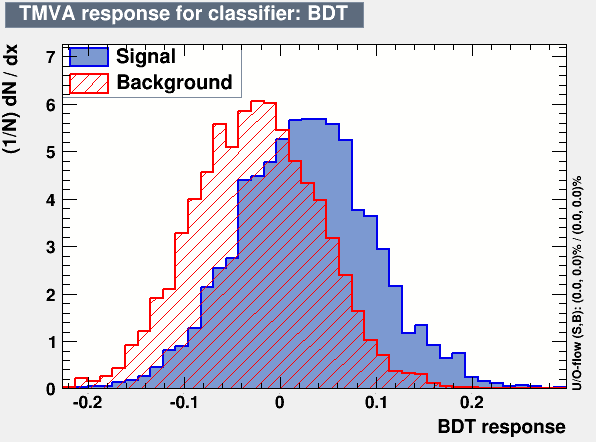
\includegraphics[width=\linewidth]{BDT_t_A}
	\caption{Plot for BDT (test sample) from TMVA analysis in region A}
\endminipage\hfill
\minipage{.5\textwidth}
	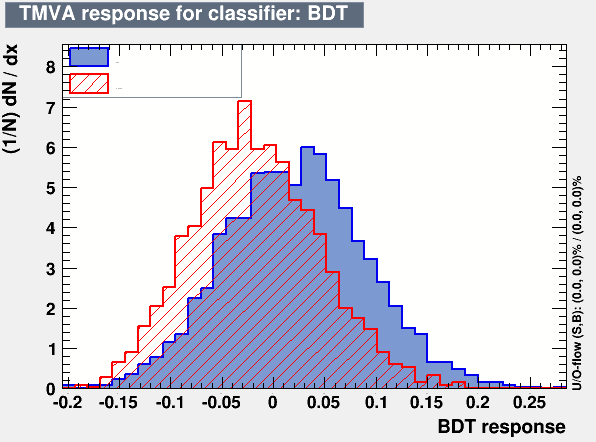
\includegraphics[width=\linewidth]{BDT_t_B}
	\caption{Plot for BDT(test sample) from TMVA analysis in region B} 
\endminipage\hfill
\end{figure}


\begin{figure}[!htb]
\minipage{.5\textwidth}
	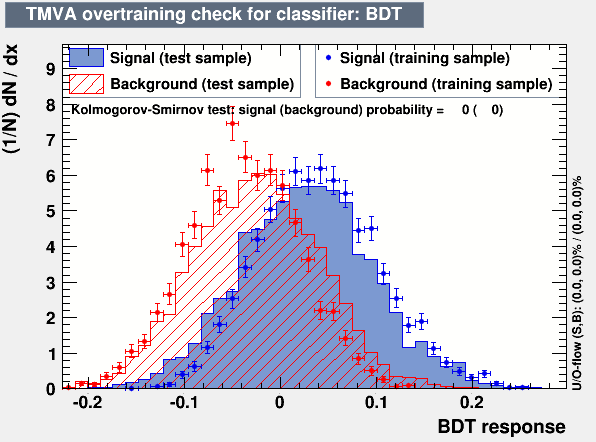
\includegraphics[width=\linewidth]{BDT_tt_A}
	\caption{BDT(test and training) from TMVA analysis in region A}
\endminipage\hfill
\minipage{.5\textwidth}
	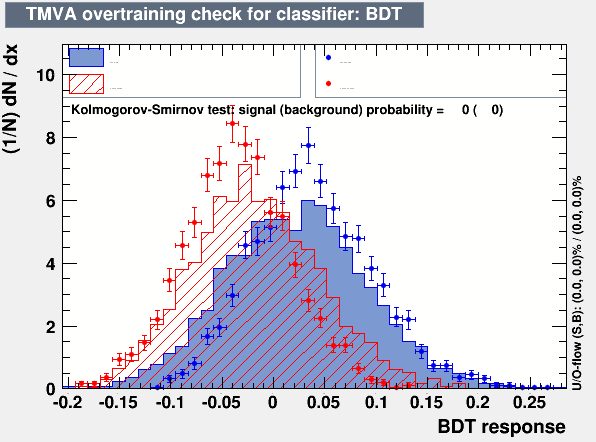
\includegraphics[width=\linewidth]{BDT_tt_B}
	\caption{BDT(test and training) from TMVA analysis in region B}
\endminipage\hfill
\end{figure}

%\newpage
%Plots for Background rejection(Spin0m) vs Signal efficiency(Spin0p)\\
%\begin{figure}[!htb]
%\minipage{.5\textwidth}
         %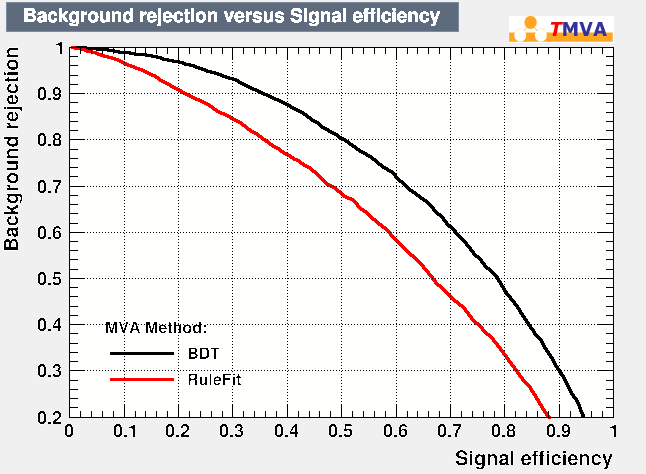
\includegraphics[width=\linewidth]{bksig_roc_u}
         %\caption{Background rejection vs signal efficiency curve for unweighted}
 %\endminipage\hfill
 %\minipage{.5\textwidth}
         %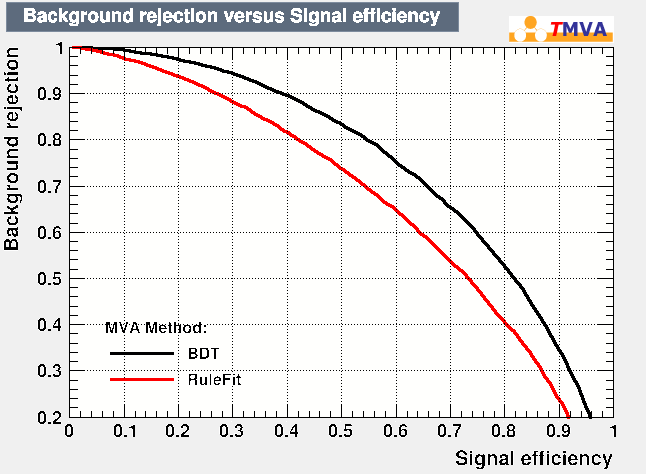
\includegraphics[width=\linewidth]{bksig_roc_w}
         %\caption{Background rejection vs signal efficiency curve for weighted}
 %\endminipage\hfill
 %\end{figure}

\end{document}
